\documentclass[a4paper,11pt,twoside]{article}

\usepackage{amsmath,amssymb}             % AMS Math
\usepackage[english]{babel}
\usepackage[utf8]{inputenc}
%\usepackage[T1]{fontenc}
\usepackage[left=1.1in,right=0.9in,top=0.4in,bottom=0.7in,includefoot,includehead,headheight=25.9pt]{geometry}
%\usepackage{verbatim}

%	Boolean includes
%\usepackage[utf8]{inputenc}
%\usepackage[T1]{fontenc}
%\usepackage{fixltx2e}
%\usepackage{graphicx}
\usepackage{longtable}
\usepackage{float}
\usepackage{wrapfig}
\usepackage{soul}
%\usepackage{t1enc}
\usepackage{textcomp}
%\usepackage{marvosym}
\usepackage{wasysym}
\usepackage{latexsym}
\usepackage{amssymb}
%\usepackage{hyperref}
%\usepackage{amsmath}
\tolerance=1000
\providecommand{\alert}[1]{\textbf{#1}}

%	Resources includes
%\usepackage{multicol}
%\usepackage[hang, bf]{caption}
%\usepackage[automark]{scrpage2}
%\usepackage[utf8]{inputenc}
%\usepackage[american]{babel}
%\usepackage{graphicx}%[pdftex]
%\usepackage[
%    %pdftex,
%    a4paper,
%    bookmarks,
%    bookmarksopen=true,
%    bookmarksnumbered=true,
%    pdfauthor={Christian Diener},
%    pdftitle={},
%    colorlinks,
%    linkcolor=black,
%    citecolor=black,
%    urlcolor=black
%]{hyperref}
\usepackage[svgnames]{xcolor}
%The following two lines import the AMS math packages and its environments
%The option intlimits forces the limits of an integral to be drawn above and
%below the integral sign
%and NOT shifted to the right
%\usepackage[intlimits]{amsmath}
%\usepackage{amsfonts}
%usepackage{amssymb}
%\usepackage{listings}
%\usepackage[round]{natbib}

%\usepackage{abstract}

\newcommand{\dt}[1]{\frac{d [\mathrm{#1}]}{dt}}
\newcommand{\sdt}[1]{\frac{d #1}{dt}}
\newcommand{\C}[1]{[\mathrm{#1}]}
\DeclareMathOperator{\im}{\mathfrak{Im}}
\DeclareMathOperator{\re}{\mathfrak{Re}}
\DeclareMathOperator{\R}{\mathbb{R}}
\DeclareMathOperator{\id}{\mathbf{id}}
\DeclareMathOperator{\Prob}{\mathbb{P}}
\DeclareMathOperator{\St}{\mathbf{S}(t)}
\DeclareMathOperator{\Div}{\mathbf{div}}
\DeclareMathOperator{\Var}{\mathbf{Var}}
\usepackage{subfig}


%	Copasi includes
%\usepackage{epsfig}
\usepackage{chemarr}
%\usepackage{graphicx}
%\usepackage{hyperref}
%\usepackage{pdfpages}



\renewcommand{\baselinestretch}{1.05}

% Table of contents for each chapter

%\usepackage[nottoc, notlof, notlot, notbib]{tocbibind}
%\usepackage[english]{minitoc}
%\setcounter{minitocdepth}{2}
%\mtcindent=15pt
% Use \minitoc where to put a table of contents

%\usepackage{aecompl}

% Glossary / list of abbreviations

\usepackage[intoc]{nomencl}
\renewcommand{\nomname}{List of Abbreviations}

\makenomenclature

% My pdf code

\usepackage{ifpdf}

\ifpdf
  \usepackage[pdftex]{graphicx}
  \DeclareGraphicsExtensions{.jpg}
  \usepackage[pagebackref,hyperindex=true]{hyperref}
\else
  \usepackage{graphicx}
  \DeclareGraphicsExtensions{.ps,.eps}
  \usepackage[a4paper,dvipdfm,pagebackref,hyperindex=true]{hyperref}
\fi

\graphicspath{{.}{images/}}

% nicer backref links
\renewcommand*{\backref}[1]{}
\renewcommand*{\backrefalt}[4]{%
\ifcase #1 %
(Not cited.)%
\or
(Cited on page~#2.)%
\else
(Cited on pages~#2.)%
\fi}
\renewcommand*{\backrefsep}{, }
\renewcommand*{\backreftwosep}{ and~}
\renewcommand*{\backreflastsep}{ and~}

% Colors, Links in pdf
\usepackage{color}
\definecolor{linkcol}{rgb}{0,0,0.4} 
\definecolor{citecol}{rgb}{0.5,0,0} 
\definecolor{darkblue}{rgb}{0., 0., .5}
\definecolor{blue}{rgb}{0., 0., 1}
\definecolor{darkred}{rgb}{.5, 0., 0.}
\definecolor{red}{rgb}{1, 0., 0.}
\definecolor{darkgreen}{rgb}{0., .5, 0.}
\definecolor{green}{rgb}{0., 1., 0.}
\definecolor{darkgray}{rgb}{.25, .25, .25}
\definecolor{lightgray}{rgb}{.70, .70, .70}
\definecolor{gray}{rgb}{0.5, 0.5, 0.5}

% Change this to change the informations included in the pdf file

% See hyperref documentation for information on those parameters

\hypersetup
{
bookmarksopen=true,
pdftitle="Fachkurs Modellierung biologischer Systeme",
pdfauthor="Friedemann Uschner (Ed.)", 
pdfsubject="Fachkurs script - November 2016", %subject of the document
%pdftoolbar=false, % toolbar hidden
pdfmenubar=true, %menubar shown
pdfhighlight=/O, %effect of clicking on a link
colorlinks=true, %couleurs sur les liens hypertextes
%pdfpagemode=None, %aucun mode de page
pdfpagelayout=SinglePage, %ouverture en simple page
pdffitwindow=true, %pages ouvertes entierement dans toute la fenetre
linkcolor=linkcol, %couleur des liens hypertextes internes
citecolor=citecol, %couleur des liens pour les citations
urlcolor=linkcol %couleur des liens pour les url
}

% definitions.
% -------------------

\setcounter{secnumdepth}{3}
\setcounter{tocdepth}{2}

% Some useful commands and shortcut for maths:  partial derivative and stuff

\newcommand{\pd}[2]{\frac{\partial #1}{\partial #2}}
\def\abs{\operatorname{abs}}
\def\argmax{\operatornamewithlimits{arg\,max}}
\def\argmin{\operatornamewithlimits{arg\,min}}
\def\diag{\operatorname{Diag}}
\newcommand{\eqRef}[1]{(\ref{#1})}

\usepackage{rotating}                    % Sideways of figures & tables
%\usepackage{bibunits}
%\usepackage[sectionbib]{chapterbib}          % Cross-reference package (Natural BiB)
%\usepackage{natbib}                  % Put References at the end of each chapter
                                         % Do not put 'sectionbib' option here.
                                         % Sectionbib option in 'natbib' will do.
\usepackage{fancyhdr}                    % Fancy Header and Footer

% \usepackage{txfonts}                     % Public Times New Roman text & math font
  
%%% Fancy Header %%%%%%%%%%%%%%%%%%%%%%%%%%%%%%%%%%%%%%%%%%%%%%%%%%%%%%%%%%%%%%%%%%
% Fancy Header Style Options

\pagestyle{fancy}                       % Sets fancy header and footer
\fancyfoot{}                            % Delete current footer settings

%\renewcommand{\chaptermark}[1]{         % Lower Case Chapter marker style
%  \markboth{\chaptername\ \thechapter.\ #1}}{}} %

%\renewcommand{\sectionmark}[1]{         % Lower case Section marker style
%  \markright{\thesection.\ #1}}         %

\fancyhead[LE,RO]{\bfseries\thepage}    % Page number (boldface) in left on even
% pages and right on odd pages
\fancyhead[RE]{\bfseries\nouppercase{\leftmark}}      % Chapter in the right on even pages
\fancyhead[LO]{\bfseries\nouppercase{\rightmark}}     % Section in the left on odd pages

\let\headruleORIG\headrule
\renewcommand{\headrule}{\color{black} \headruleORIG}
\renewcommand{\headrulewidth}{1.0pt}
\usepackage{colortbl}
\arrayrulecolor{black}

\fancypagestyle{plain}{
  \fancyhead{}
  \fancyfoot{}
  \renewcommand{\headrulewidth}{0pt}
}

% \usepackage{algorithm}
% \usepackage[noend]{algorithmic}

%%% Clear Header %%%%%%%%%%%%%%%%%%%%%%%%%%%%%%%%%%%%%%%%%%%%%%%%%%%%%%%%%%%%%%%%%%
% Clear Header Style on the Last Empty Odd pages
\makeatletter

\def\cleardoublepage{\clearpage\if@twoside \ifodd\c@page\else%
  \hbox{}%
  \thispagestyle{empty}%              % Empty header styles
  \newpage%
  \if@twocolumn\hbox{}\newpage\fi\fi\fi}

\makeatother
 
%%%%%%%%%%%%%%%%%%%%%%%%%%%%%%%%%%%%%%%%%%%%%%%%%%%%%%%%%%%%%%%%%%%%%%%%%%%%%%% 
% Prints your review date and 'Draft Version' (From Josullvn, CS, CMU)
\newcommand{\reviewtimetoday}[2]{\special{!userdict begin
	/bop-hook{gsave 20 710 translate 45 rotate 0.8 setgray
      /Times-Roman findfont 12 scalefont setfont 0 0   moveto (#1) show
      0 -12 moveto (#2) show grestore}def end}}
% You can turn on or off this option.
% \reviewtimetoday{\today}{Draft Version}
%%%%%%%%%%%%%%%%%%%%%%%%%%%%%%%%%%%%%%%%%%%%%%%%%%%%%%%%%%%%%%%%%%%%%%%%%%%%%%% 

\newenvironment{maxime}[1]
{
\vspace*{0cm}
\hfill
\begin{minipage}{0.5\textwidth}%
%\rule[0.5ex]{\textwidth}{0.1mm}\\%
\hrulefill $\:$ {\bf #1}\\
%\vspace*{-0.25cm}
\it 
}%
{%

\hrulefill
\vspace*{0.5cm}%
\end{minipage}
}

%\let\minitocORIG\minitoc
%\renewcommand{\minitoc}{\minitocORIG \vspace{1.5em}}

\usepackage{multirow}
%\usepackage{slashbox}

\newenvironment{bulletList}%
{ \begin{list}%
	{$\textbullet$}%
	{\setlength{\labelwidth}{25pt}%
	 \setlength{\leftmargin}{30pt}%
	 \setlength{\itemsep}{\parsep}}}%
{ \end{list} }
% set up itemization lists to display the bullet points correctly - for whatever reason not working properly
% (getting bullet points only on the second level of itemization)
%\usepackage{enumitem}
%\setlist[itemize,1]{label={\fontfamily{cmr}\fontencoding{T1}\selectfont\textbullet}}

\newtheorem{definition}{Definition}
\renewcommand{\epsilon}{\varepsilon}
%\usepackage{hhline,float,booktabs}
\newcommand*{\thickhline}{\noalign{\hrule height 1pt}}
% centered page environment

\newenvironment{vcenterpage}
{\newpage\vspace*{\fill}\thispagestyle{empty}\renewcommand{\headrulewidth}{0pt}}
{\vspace*{\fill}}

% Marvin new commands
\usepackage{epsfig}
\usepackage{chemarr}
\newcommand{\beq }{\begin{equation}} 
\newcommand{\eeq }{\end{equation}} 
\newcommand{\Ii }{I_{\mbox{\scriptsize\it Ion}}} 
\newcommand{\Iii }{I_{\mbox{\scriptsize\it Ion},i}} 
\newcommand{\wi }{w_{\infty}}
\newcommand{\md }{\text{d}}
\newcommand{\code}[1]{\begin{verbatim}#1\end{verbatim}}
\renewcommand{\baselinestretch}{1.2}
\renewcommand{\arraystretch}{1.2}




% weitere Einfügungen
\setcounter{tocdepth}{1}
\usepackage{framed}
\usepackage{setspace}
\usepackage{pdfpages}
\usepackage{color}

\hyphenation{tem-pe-ra-tures hy-per-po-la-ri-sing}

\usepackage{comment}

% Matlab chapter
\usepackage[numbered]{mcode}
\usepackage{listings}

% [edit: for matlab code to work, this needs to be excluded:]
%fancyvr bconfig
% \lstset{numbers=left, numberblanklines=false, 
% numberstyle=\color{gray}\scriptsize\ttfamily, extendedchars=true, 
% language=Python, keywordstyle=\bfseries\color{darkblue}, 
% identifierstyle=\mdseries, stringstyle=\color{darkred}, tabsize=4, 
% basicstyle=\scriptsize\ttfamily, columns=flexible, showtabs=false, 
% showspaces=false, showstringspaces=false, morecomment=[s]
% [\upshape\color{darkgreen}]{/**}{*/}, postbreak={\dots}, prebreak={\dots}, 
% breakindent=5pt, breaklines, captionpos=b}
% \newcommand*\command[1][]{\medskip%
% {\noindent}\allowbreak\colorbox[rgb]{.80,.80,.80}
% {\allowbreak\makebox[\linewidth][l]{\begin{minipage}[c]
% {\linewidth}\allowbreak\texttt{#1}\end{minipage}}}\bigskip}

\setlength{\parindent}{0cm}
%\usepackage{enumitem}
%\setlist[itemize,1]{label={\fontfamily{tnr}\fontencoding{T1}\selectfont\textbullet}}

\renewcommand{\familydefault}{\sfdefault}
\setcounter{tocdepth}{2}

\begin{document}

\thispagestyle{empty}
 \begin{center}
 \textbf{ \Huge Kinetic Modeling With Copasi}\\\vspace{0.2cm}
Fachkurs Theoretische Biophysik, WS 2016/17
 \end{center}

\vspace{3cm}

Copasi\footnote{Hoops S, Sahle S, Gauges R, Lee C, Pahle J, Simus N,
 Singhal M, Xu I, Mendes P, Kummer U. \textit{COPASI: a COmplex
  PAthway SImulator.} \textbf{Bioinformatics} 2006; 83:3067--3074}
is a software application for simulation and analysis of biochemical
networks. It is available for MS Windows, Linux and Mac OS X\footnote{available  at \url{http://www.copasi.org}}  and can
import and export models in the standardized SBML format. This introductory course will explain how to implement simple biochemical models as systems of ordinary differential equations in the graphical user interface (GUI ) of Copasi. The major capabilities of Copasi for the analysis of the implemented model will be presented. The introduction is followed by some hands on exercises with different models and functionalities.
%COPASI comes in two versions. One with a GUI for interactive work and one without a GUI for batch processing of model files. In this course we will focus on the former one.\\
\vspace{1cm}\\
This accompanying document is a Copasi reference rather than a manual. A very detailed and
easy  to  understand  Copasi  manual can  be  acessed on 
\url{http://www.copasi.org}. If you encounter any problems with Copasi that cannot
be answered in this course, you can also check the User Support Forum
there. Online tutorials are available at:\\
\url{http://copasi.org/Support/Video_Tutorials/}\\
\url{http://vimeo.com/user3657452/videos/sort:date}

\newpage
\tableofcontents


\newpage
\section{Copasi}
A model consists of species and interactions between species. Copasi allows to compile these elements in a structured way. Different aspects of the model as well as Copasi functions are browsed via a menu on the left side of the main window and edited inside the main window (see Figure \ref{fig:MainWindow}). Plots for different tasks are issued in additional windows. We will walk through some of the submenus:

\begin{figure}[b!]
 \centering
 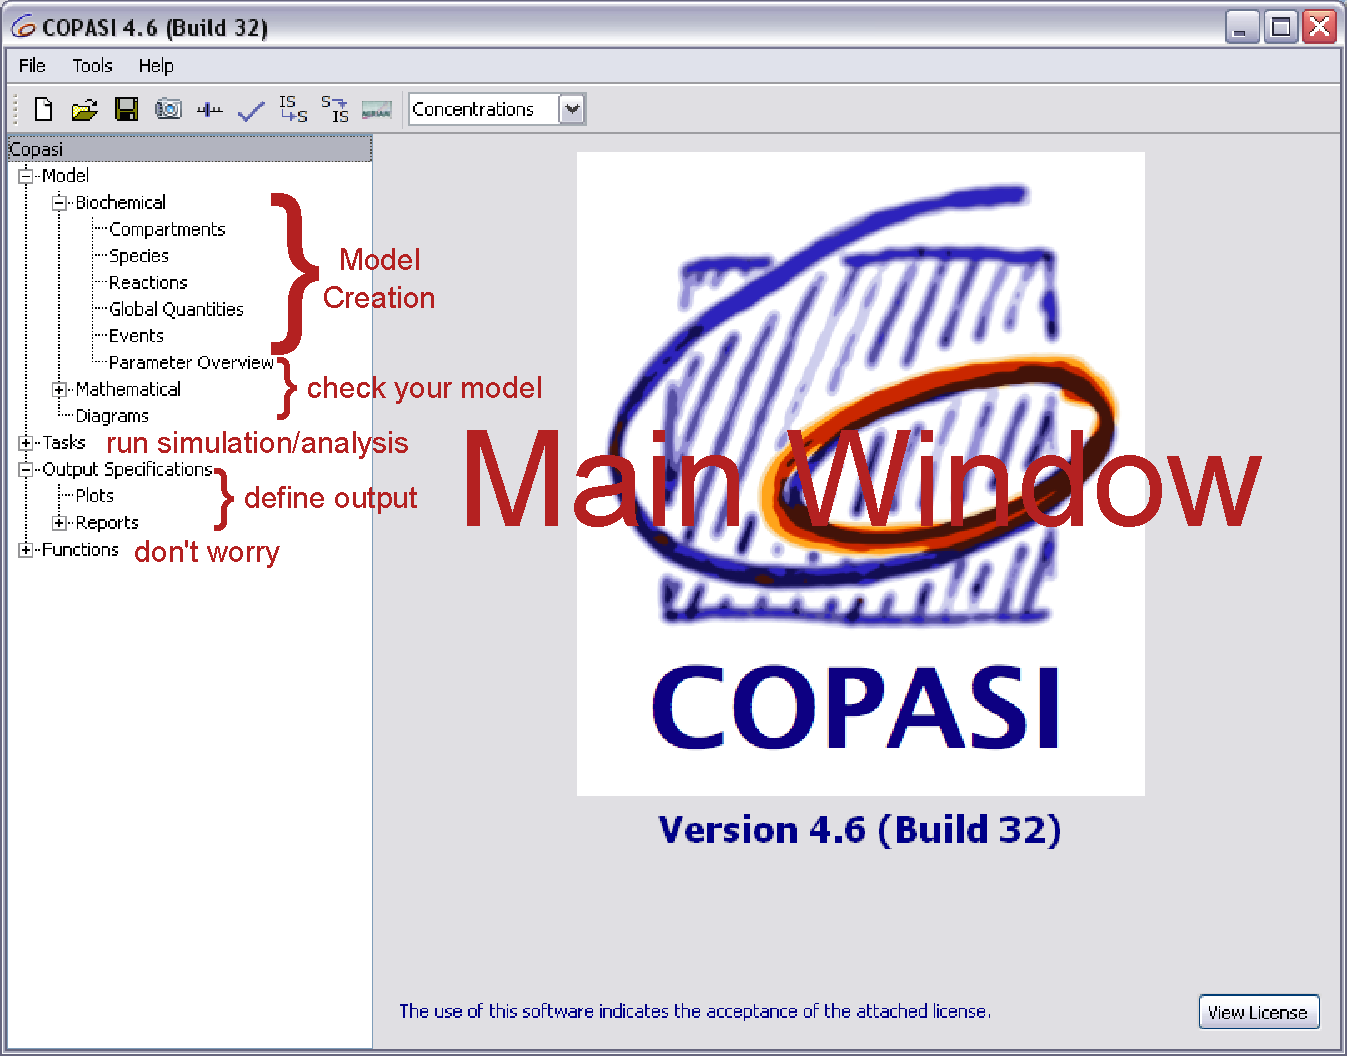
\includegraphics[width=09cm]{Pictures/CopasiMainWindow.pdf}
 \caption{\footnotesize Copasi upon start-up. The function of different submenus is indicated.  The main window will display different contents depending on the active submenu.}
 \label{fig:MainWindow}
\end{figure}

\begin{itemize}
\item Model  - \textit{describe model,  set units, see }\textbf{\ref{sub:Model}}
 \begin{itemize}
 \item  Biochemical   -  \textit{edit  model,  see } \textbf{\ref{sub:Biochem1}}
  \begin{itemize}
  \item Compartments
  \item Species
  \item  Reactions  - \textit{define  reactions,   see }\textbf{\ref{sub:Biochem2}}
  \item Global Quantities  - \textit{parameters and assignment  variables, see }\textbf{\ref{sub:Biochem3}}
  \item  Events  -  \textit{discrete  events,  see }\textbf{\ref{sub:Biochem4}}
  \item Parameter Overview - \textit{view parameters}
  \end{itemize}
 \item Mathematical - \textit{view equations and matrices}
  \begin{itemize}
  \item Differential Equations - \textit{view model equations,  see }\textbf{\ref{sub:DiffEq}}
  \item Matrices - \textit{view stoichiometry}
 \item Diagrams - \textit{create simple network diagrams of your model}
  \end{itemize}
 \end{itemize}
\item Tasks - \textit{model simulation and functional analyses, see }\textbf{\ref{sub:Tasks}}
 \begin{itemize} 
 \item Steady State -  \textit{find and analyze the steady state of the model, see }\textbf{\ref{sub:TC}}
 \item Time  Course -  \textit{simulate the  model, see }\textbf{\ref{sub:TC}}
 \item  Parameter Scan  - \textit{simulate  the  model varying parameters, see }\textbf{\ref{sub:PS}}
 \item other advanced tasks: Parameter Estimation, Optimzation, Linear noise approximation...
 \end{itemize}
\item Output Specifications
 \begin{itemize}
 \item Plots - \textit{add, change or remove plots} \textbf{\ref{sub:Plots}}
\item Reports - \textit{add, change or remove reports of tasks to be saved externally} \textbf{\ref{sub:Reports}}
 \end{itemize}
\item Functions - \textit{add,  change or remove  functions for reaction rate laws} \textbf{\ref{sub:funct}}
\item Units - \textit{Predefined units that can be used in the model to ensure consistency}

\end{itemize}

An important and ubiquitous \textbf{button} is the one with the \textbf{Copasi icon} on it ("curly button"). It is used \textbf{to select} previously defined \textbf{model entities} in different contexts.\\
Another important  concept in fields that  require free input:~{\color{blue}\textbf{Blue}} background  means (formally) correct.{ \color{red}\textbf{Red}} background indicates formal mistakes.


\section{Creating a Model}
\subsection{Model}
\label{sub:Model}
Define  model  \textbf{units}  and \textbf{describe}  the  model (e.g. leave notes to remember what you want to do).
\subsection{Biochemical - compartments and species}
\label{sub:Biochem1}
Define model variables and the compartments that contain them.\\
\textbf{Fixed species have a fixed particle number. Compartment volume changes will change their concentration!}
\subsection{Biochemical - reactions}
\label{sub:Biochem2}
Define reactions (Figure \ref{fig:Reactions}).  Chemical equations use \textbf{'+' '-$>$' '=' ';' '*' } where \textbf{each operator is separated by blanks}. Any name in the chemical equation that is neither an operator nor a species will \textbf{create a new species}. Depending on the stoichiometry of the chemical equation, a kinetic rate law can be chosen from the drop-down list of possible kinetic laws. It is also possible to create a specific new kinetic law.\\
The bottom part gives an overview of the assignments of numbers, species and parameters to the kinetic law.

\begin{figure}[htb]
 \centering
 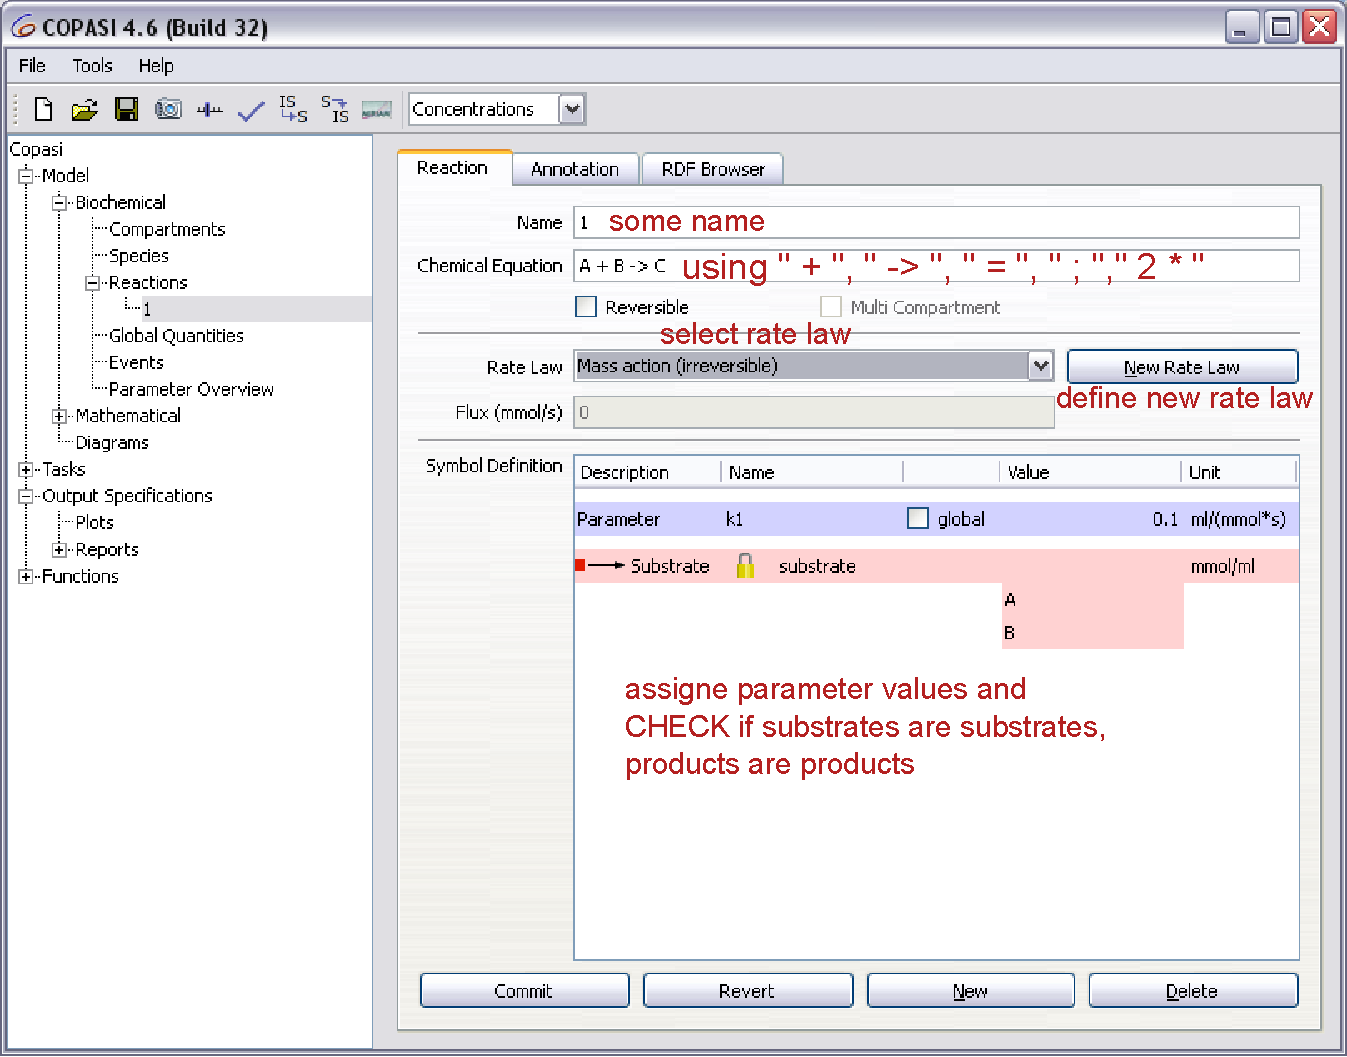
\includegraphics[width=09cm]{Pictures/CopasiReactions2.pdf}
 \caption{\footnotesize Creating reactions in Copasi.}
 \label{fig:Reactions}
\end{figure}

\subsection{Biochemical - global quantities}
\label{sub:Biochem3}
Define global parameters as \textbf{fixed} values, \textbf{assignment} variables or \textbf{ODE}. Only if the moedl parameters are defined here, they will be accessible to the tasks manipulating parameters such as Parameter Scan or Parameter Estimation.\\
In the case of \textbf{assignment} variables, the empty field is used to enter the \textbf{right hand side} of the equation determining the assignment  variable  (see  Figure  \ref{fig:GQ}). Use  the \textbf{Copasi-button} to select model variables to be used in the
equation. 

\begin{figure}[b!]
 \centering
 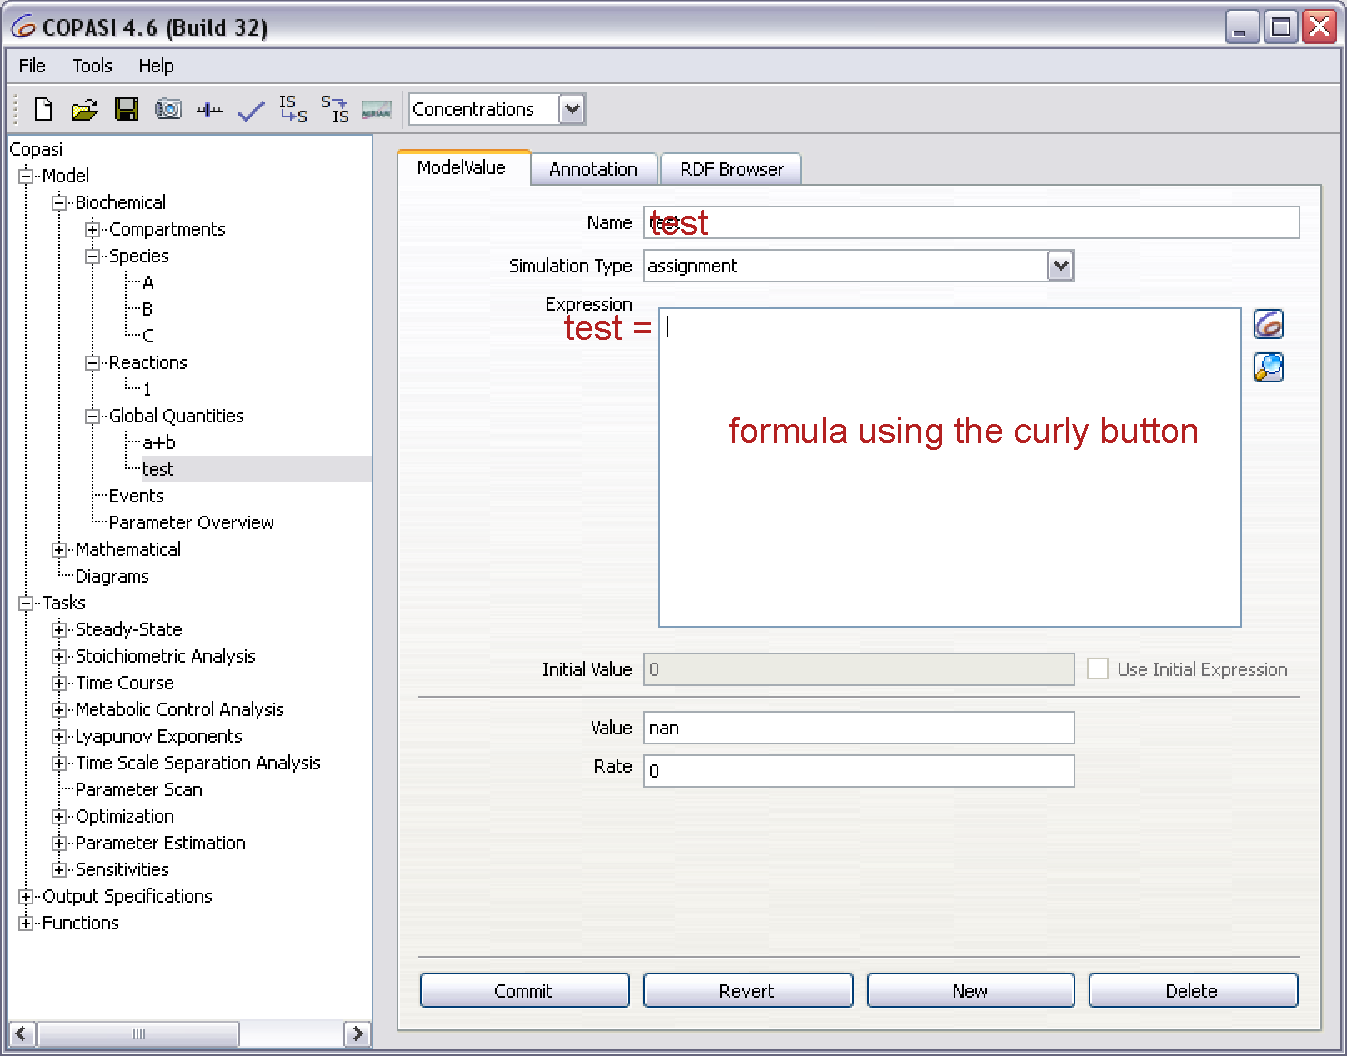
\includegraphics[width=09cm]{Pictures/CopasiGQ.pdf}
 \caption{\footnotesize Creating assignment quantities in Copasi.}
 \label{fig:GQ}
\end{figure}

\subsection{Biochemical - events}
\label{sub:Biochem4}
Events are used to define assignments that happen \textbf{once} a certain condition is fulfilled. This could for example be the increase of a concentration across a certain threshold or a specific time. Such trigger expressions can be defined using model variables (via the curly button) and relation operators '\textbf{lt}' (less than), '\textbf{le}' (less equal), '\textbf{gt}' (greater than), '\textbf{ge}' (greater equal), '\textbf{eq}' (equal).\\
The curly button is also used to define event targets, \textit{e.g.} what happens when the event is triggered. Be careful to not leave any empty assignments, when changing event targets, as this causes errors.

\subsection{Functions}
\label{sub:funct}
Functions are used to define rate laws for the model reactions. There is a number of predefined rate laws that can't be changed. If you define additional rate laws, they are stored here. If a function is in use in a reaction it  can only be modified to some extent!\\
\textbf{Formula: }The formula can be entered freely using a wide range of operators. Just make sure you are mathematically consistent, \textit{e.g} never divide by zero. The names of the species and parameters in the function do not need to match the names of the reacting  species. They are mapped to the reacting species for each reaction in the Biochemical - reactions section.\\
\textbf{Function type:} Checking \textbf{General} puts you on the safe side.\\
\textbf{Parameters:} Here, you define which name in the formula corresponds to which type of model entity (substrate, product, modifier, parameter,...). Make sure that this classification  complies  with the chemical equation of the reaction you want to use this formula for (a reaction without products can not be assigned a formula that uses products).

\begin{figure}[htb]
 \centering
 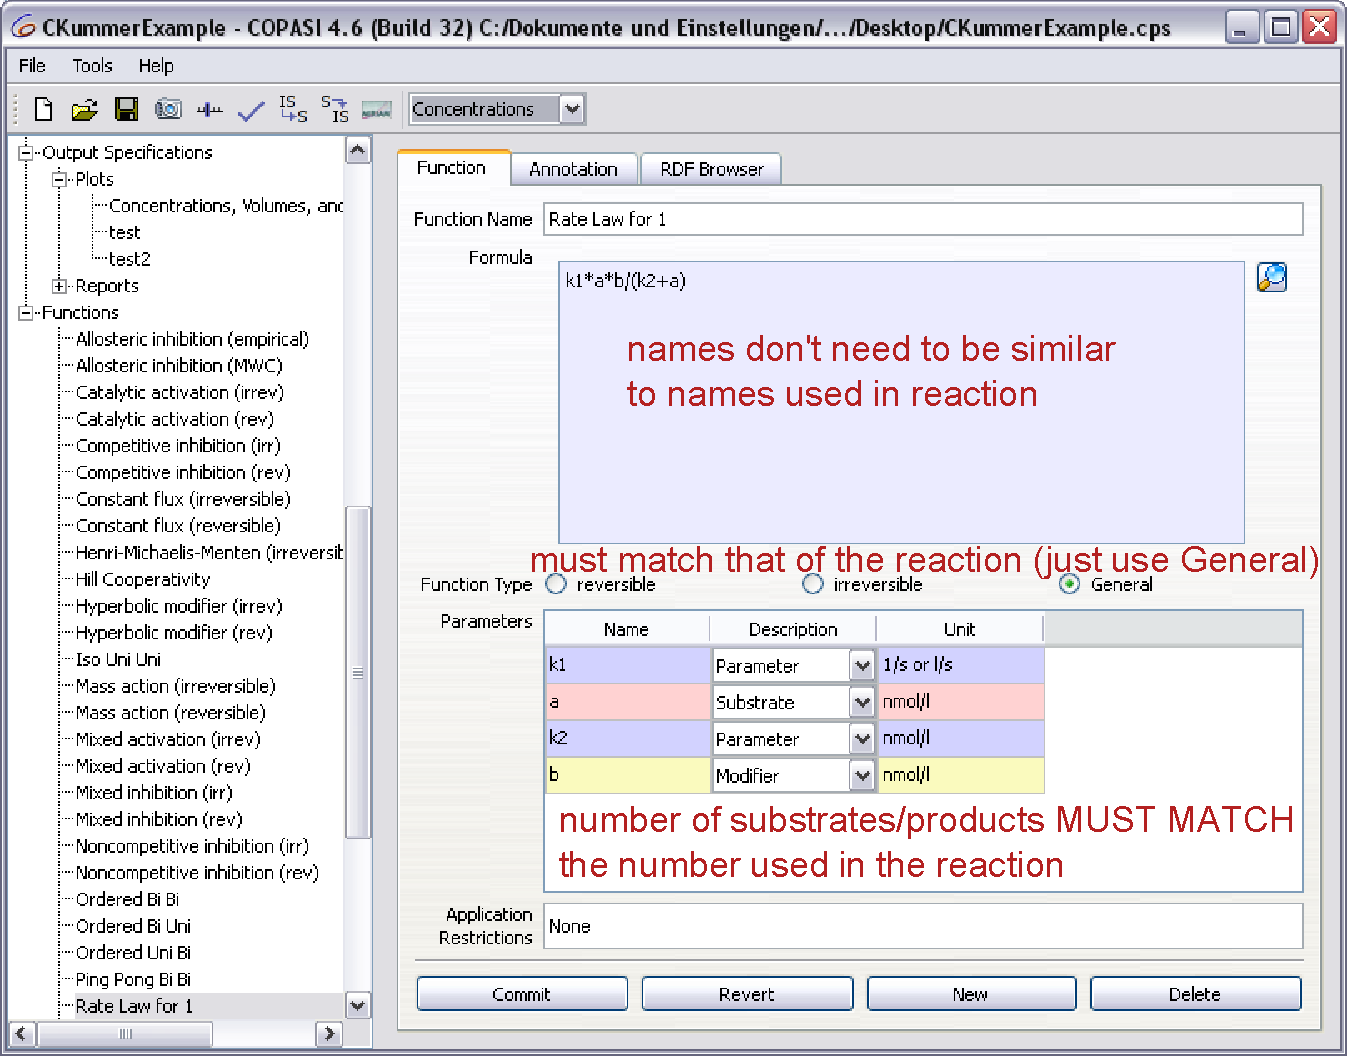
\includegraphics[width=11cm]{Pictures/CopasiFunction21.pdf}
 \caption{\footnotesize Adding a new function to Copasi.}
 \label{fig:funct}
\end{figure}

\subsection{Mathematical - Differential Equations}
\label{sub:DiffEq}
View the equations generated from the reactions and global quantities. Be sure to \textbf{check} if everything is correct. Also, notice that most reaction rates take the \textbf{volume of the  containing compartment} into account. \textbf{Transport reactions} between compartments don't.


\newpage
\section{Model Analysis Using Copasi}
\subsection{Tasks}
\label{sub:Tasks}
Copasi offers a number of analyses that can help you to characterize and understand the function of your model and the underlying biological process. We will go through some of the basic tasks that cover the following topics:
\begin{itemize}
\item Time Course -  \textit{simulate your model's evolution over time, see }\textbf{\ref{sub:TC}} 
\item  Steady-State -  \textit{find and  analyze  steady state, see }\textbf{\ref{sub:ss}}
\item Parameter Scan  -  \textit{Systematically change parameters of the model and run analyses on the different parameter sets, see }\textbf{\ref{sub:PS}}
\item Sensitivities - \textit{analyze how model parameters affect  model variables, see }\textbf{\ref{sub:sens}}
\item Stoichiometric Analysis - \textit{analyze the model structure,  see }\textbf{\ref{sub:sa}}
 \begin{itemize}
 \item Elementary Modes - \textit{find pathways that can generate a steady state}
 \item Mass Conservation - \textit{check if input equals output}
 \end{itemize}
\item Metabolic Control Analysis - \textit{compute elasticities and  control coefficients, see }\textbf{\ref{sub:mca}}
\item Further advanced tasks - \textit{Lyapunov exponents, Time Scale Separation Analysis, Cross Section, Optimization, Parameter Estimation, Linear Noise Approximation -- not covered here but also cool, see the Copasi homepage for details.}
\end{itemize}

Most of these tasks do no generate graphical output, but the results are displayed in the respective 'Result' submenu.  For some, the numbers can be visualized using bar graphs there.
\textbf{Numerical results} are usually accessible via the respective \textbf{'Result' submenu}.  \textbf{Plots} in extra windows\textbf{ need to be created} before execution of the task. For more detail, see \textbf{\ref{sub:Plots}}. For more detailed numerical output, Reports in form of text files can be generated, see \textbf{\ref{sub:Reports}}.

\subsection{Plots}
\label{sub:Plots}
The results of each task can be plotted as x-y-graphs within Copasi. The plots appear as external plots in extra windows and are somewhat \textbf{independent} of the main program. Plots are not generated automatically, nor are they destroyed automatically when switching tasks. A plot receives signals from Copasi and updates accordingly, even if these signals do not make sense.
Since Copasi is in active development, new tasks (and also subtasks) are frequently added, so not all tasks might be covered in this tutorial.
\begin{figure}[t!]
 \centering
 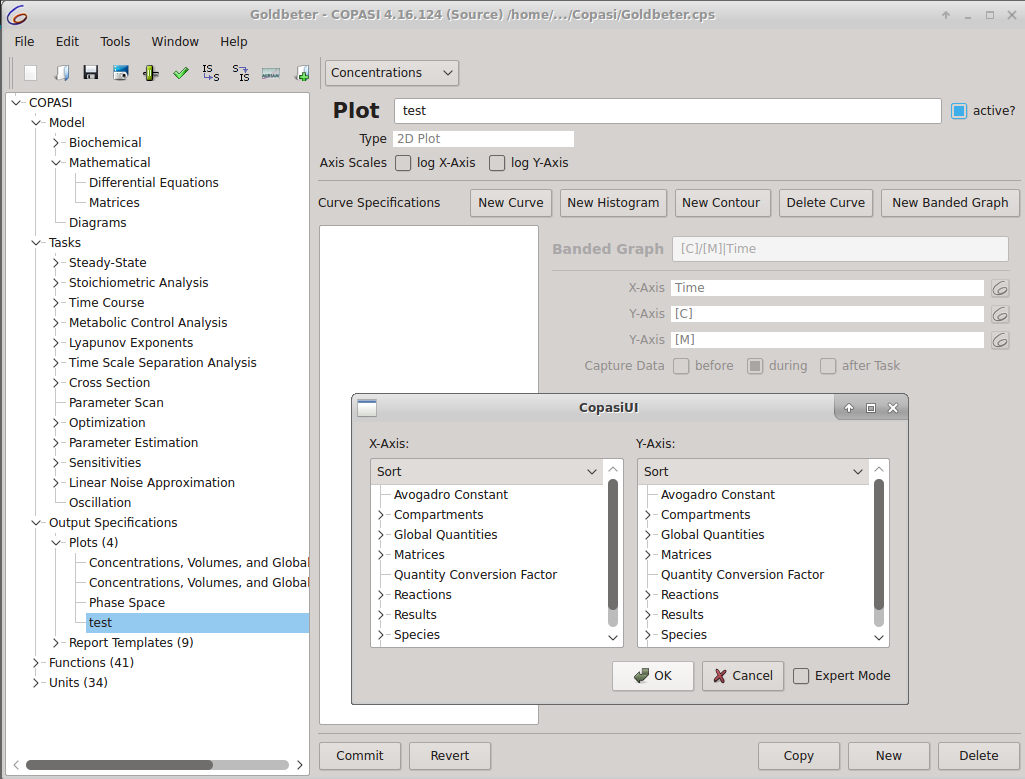
\includegraphics[width=11cm]{Pictures/Bildschirmfoto_2016-11-10_11-08-42.png}
 \caption{\footnotesize Creating a new plot.}
 \label{fig:Plot}
\end{figure}
You can also \textbf{create a new plot} with the help of the Output Assistant for each task or individually in the Plot submenu here. To do so, you can enter a new name into the last field in the list of plots. This plot can then be filled with curves, histograms, banded graphs or contour plots of model variables, which you can select using again the curly button. You have the choice to plot variables as functions of time or as functions of other variables. In case you created too many plots using the Output Assistant, this submenu is the place to \textbf{remove plots}. In a plot window, you can save the image and the raw data.

You can change a \textbf{plot's status from active to inactive}. Inactive plots are not updated. You can inactivate a plot, change the model, create a new plot and compare the results.

\subsection{Reports}
\label{sub:Reports}
For each task, a written report can be generated that summarizes all results and is saved as a text file outside of Copasi. There is a predefined report available for each task which you can activate using the Report button of each task. You can also define custom reports in the respective submenu.

\newpage
\section{Analysis and Simulation Tasks}
\subsection{Simulating the Model}
\label{sub:TC}
This task allows you to simulate the trajectories of your model species over time.\\
In the Time Series The inputs on the top determine duration of simulation and step  size.  Too many \textbf{intervals increase computation} time, \textbf{too few lead to erroneous  trajectories}.\\
Copasi can simulate deterministically and stochastically (required for systems with very low numbers of molecules), you can select the respective integration algorithm in the 'Method' tab. Each method requires parameters that control numerical precision. \textbf{Before} running \textbf{stochastic} simulations, check that the \textbf{particle numbers are low}, otherwise an error will occur.\\
To \textbf{plot} the simulation results, use the \textbf{Output  assistant button} at the bottom to create a plot, as introduced before. The plots occur in an extra window and will be updated every time a new task is executed. Therefore, you don't need to add  plotting windows for each simulation you run.\\
Be careful with the \textbf{'update model'} check-box: If marked, the initial concentrations will be overwritten with the concentrations at the end of the simulation!\\
Suggested Output Assistant Plots: the first 7.

\begin{figure}[htb]
 \centering
 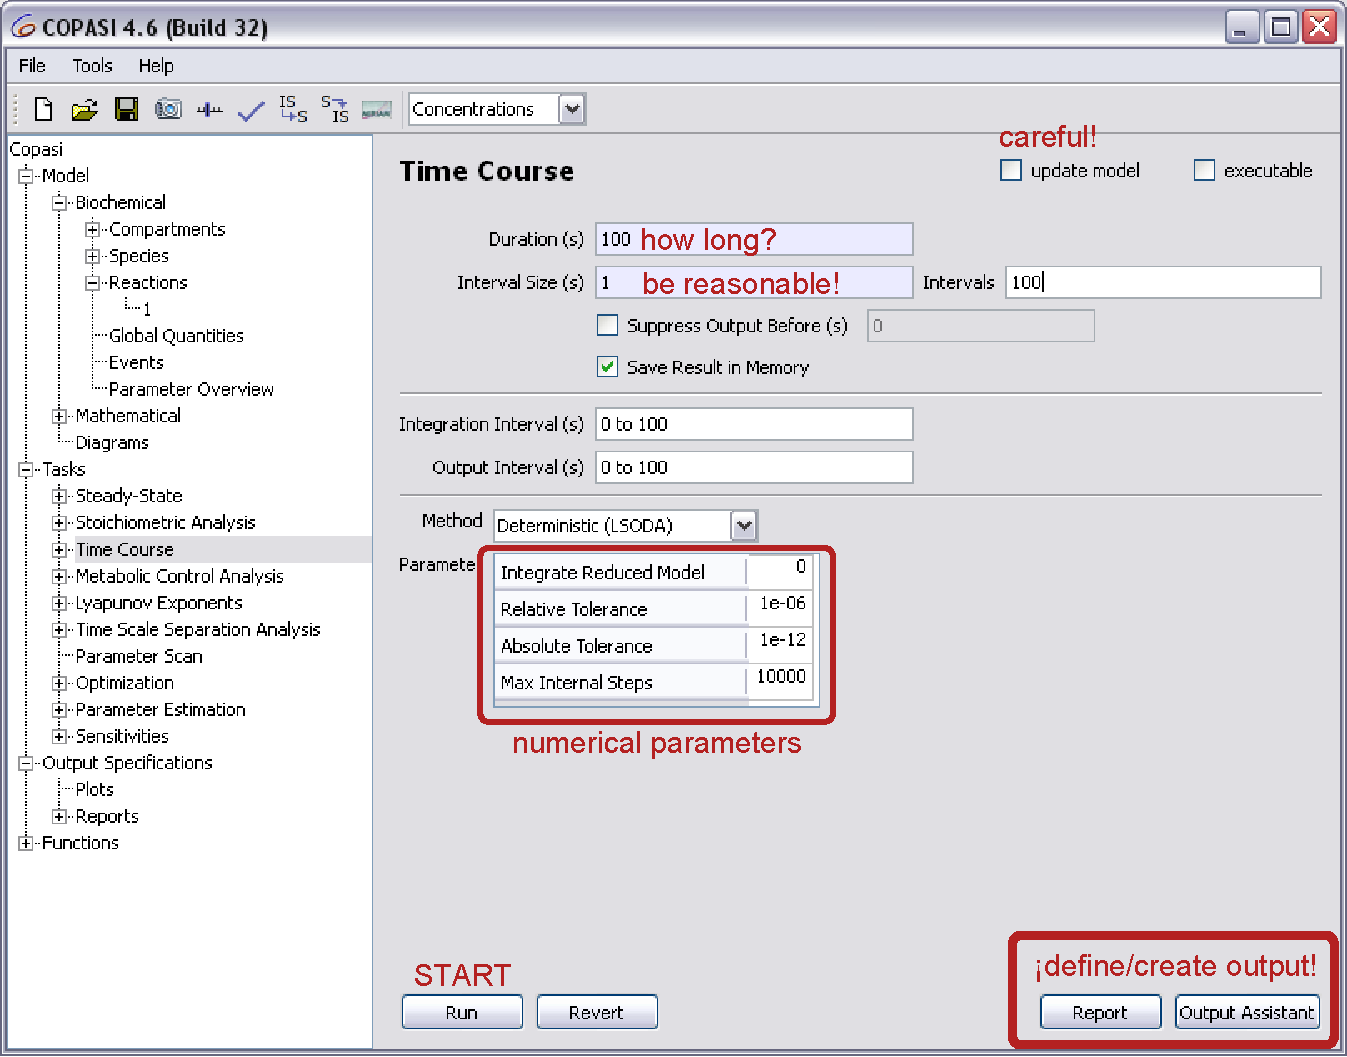
\includegraphics[width=09cm]{Pictures/CopasiSimulation.pdf}
 \caption{\footnotesize Model simulation with Copasi.}
 \label{fig:CS}
\end{figure}

\subsection{Steady-State}
\label{sub:ss}
This task numerically searches for a steady state. The stability of the steady state can be assessed using the Jacobian (the steady state is stable if all eigenvalues are negative), which is summarized in the Stability analysis.

\subsection{Parameter Scan}
\label{sub:PS}
If you now want to explore how single parameters of your model influence its time evolution you can conduct a Parameter Scan. It simulates the model after varying one or more parameters. Which parameter to scan can be selected with the curly button. You can choose between scanning a certain range for a parameter value systematically or a random distribution of parameters (with a Repeat for more than one set of random parameters). For each interval (Scan) or iteration (Repeat), Copasi will run the specified task (usually time-course, but any other task can be chosen as well). Increasing the number of scan parameters increases computation time. Also, make sure you have appropriate plots or reports to collect the outputs of the scanned simulations for each task.\\

\begin{figure}[htb]
 \centering
 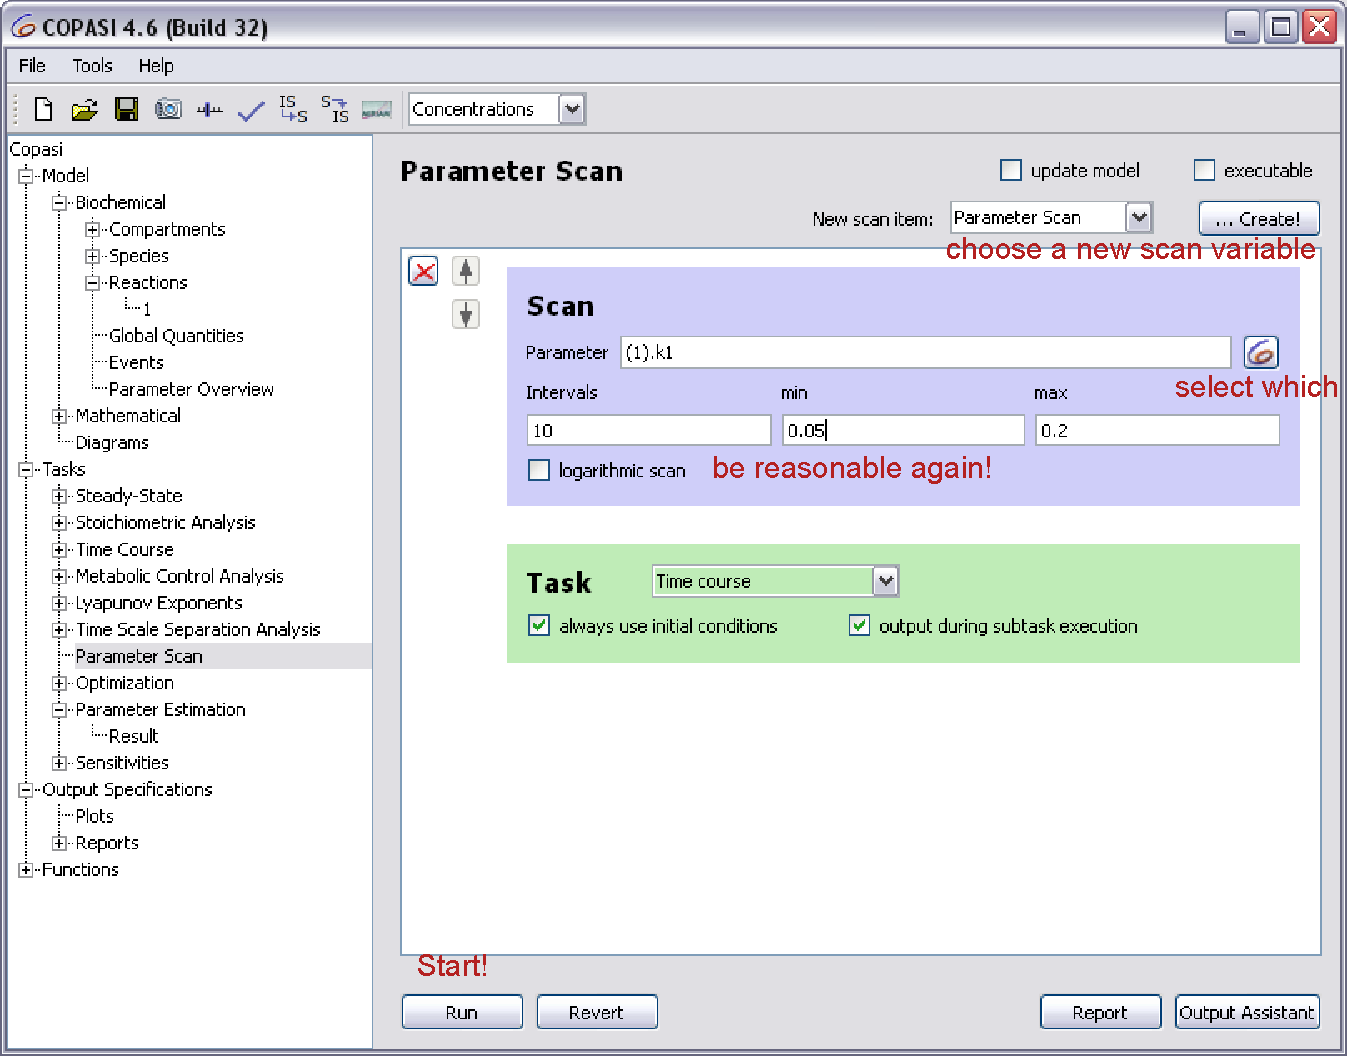
\includegraphics[width=09cm]{Pictures/ParameterScan.pdf}
 \caption{\footnotesize Parameter scan dialog}
 \label{fig:PS}
\end{figure}

\textbf{Scan:} Runs simulations varying the specified parameter using the intervals defined.\\
\textbf{Random Distribution:} Samples specified parameter from a random distribution \textbf{once}.  To run multiple times, needs a Repeat-item \textbf{before}.

\subsection{Sensitivities}
\label{sub:sens}
Sensitivities, also called response coefficients, express the direct dependence of steady state variables on parameters. The sensitivity of a flux $J_j$ to a parameter $p_m$ is given by
\begin{equation*}
 R_m^j = \frac{p_m}{J_j}\frac{\partial J_j}{\partial p_m} 
\end{equation*} 
and the sensitivity of a steady state concentration $S_i$ to a parameter $p_m$ by
\begin{equation*}
R_m^i = \frac{p_m}{S_i}\frac{\partial S_i}{\partial p_m}
\end{equation*} 
In Copasi, sensitivities are calculated as the derivatives of model variables with respect to a defined list of model entities, e.g. parameter values. Sensitivities are also calculated as global quantities of the system, i.e. indirect effects are accounted for. \\
One should consider sensitivities \textbf{scaled by the concentrations  for comparison}. \\
Although Copasi implies to compute \textbf{sensitivities for a time course}, it will only compute the sensitivities at the \textbf{last point} of the time course.

% \subsection{Parameter Estimation}
% \label{sub:PE}
% Estimate parameter values so model variables reproduce experimental
% data.
% \begin{itemize}
% \item \textbf{Data:} See Figure \ref{fig:PEdata}. Requires data in
%  tabular format. Make sure to check whether tour data is recognized
%  correctly (\textbf{Experiment Type}, \textbf{Header},
%  \textbf{Separator}). Columns in the data need to be mapped to model
%  variables. $3$ types available:
%  \begin{itemize}
%  \item \textbf{ignored}: ignore
%  \item \textbf{dependent}: the model variable chosen contributes to
% the fit
%  \item \textbf{independent}: the model variable chosen does not
% contribute but is initially set to the value in data.
%  \end{itemize}
% \item \textbf{Parameters:} See Figure \ref{fig:PEparams}. The top part
%  of the main window allows choosing parameters to be estimated. Most
%  methods are heuristic. \textbf{Decreasing the boundaries} for the
%  parameters increases the chance to find good values but requires
%  some prior knowledge.\\
%  Different methods are suitable for different problems, so
%  \textbf{try different methods}.\\
%  The \textbf{more iterations} are run, the better the
%  results. \textbf{If goodness of fit does not increase, abort}.\\
%  Suggested Output-Assistant Plots:
%  \begin{itemize}
%  \item \textbf{Progress of fit:} monitor goodness of fitted.
%  \item \textbf{Parameter Estimation  Results:} compare data and
% simulations.
%  \end{itemize}
% \end{itemize}
% In case you want to \textbf{use the parameter values found}, check the
% \textbf{'update model'} check-box \textbf{before}.
% 
% \begin{figure}[htb]
%  \centering
%  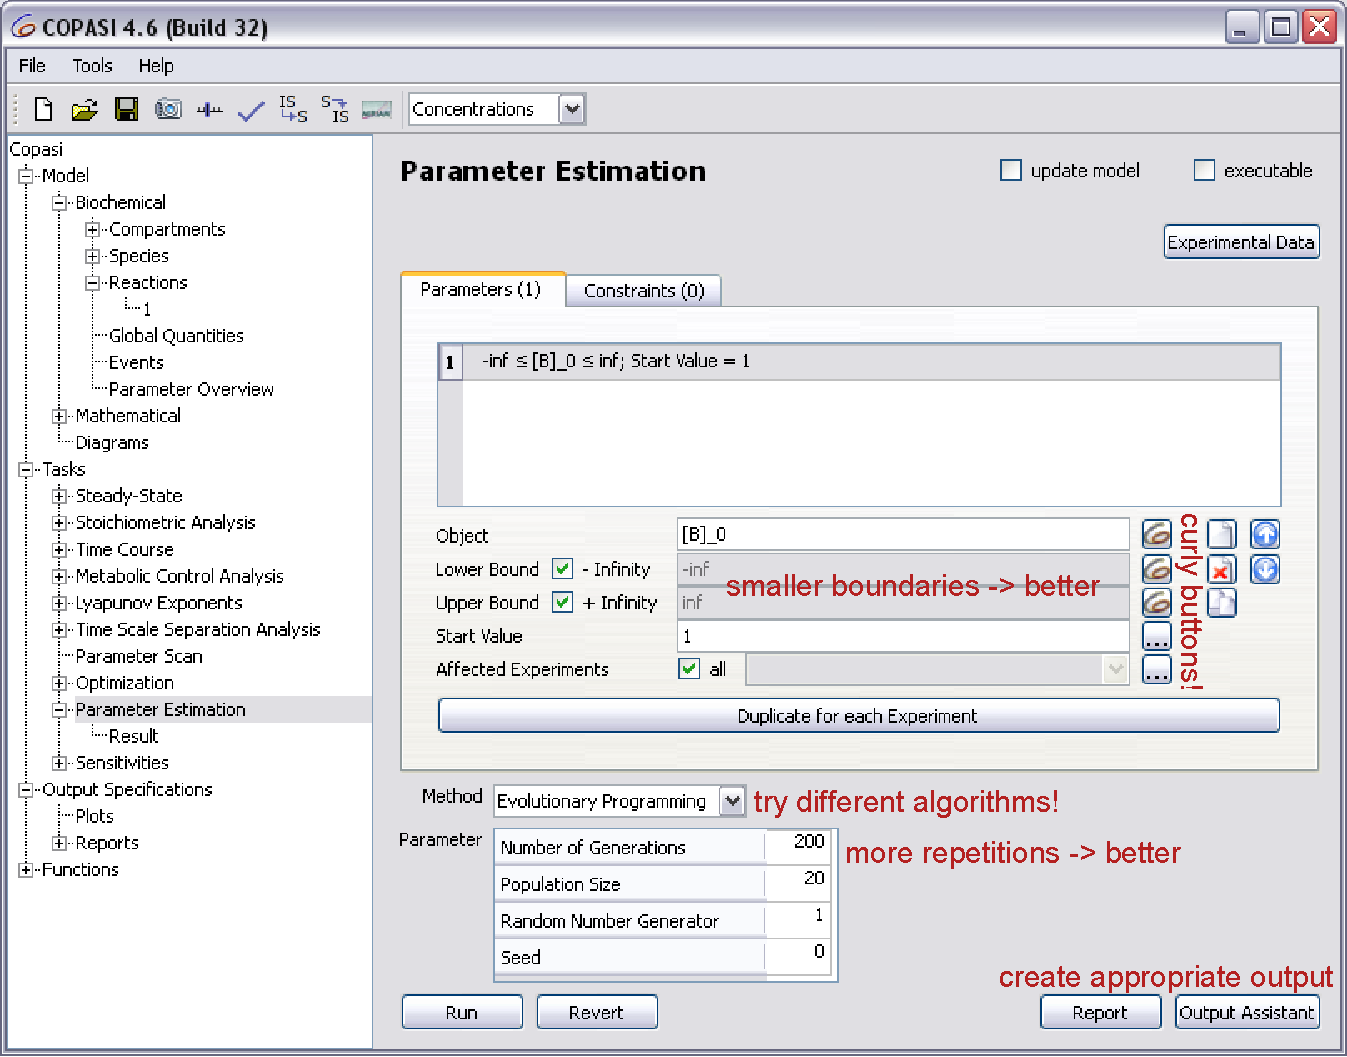
\includegraphics[width=09cm]{Pictures/ParameterEstimation_2.pdf}
%  \caption{\footnotesize Loading experimental data into Copasi}
%  \label{fig:PEparams}
% \end{figure}
% 
% \begin{figure}[htb]
%  \centering
%  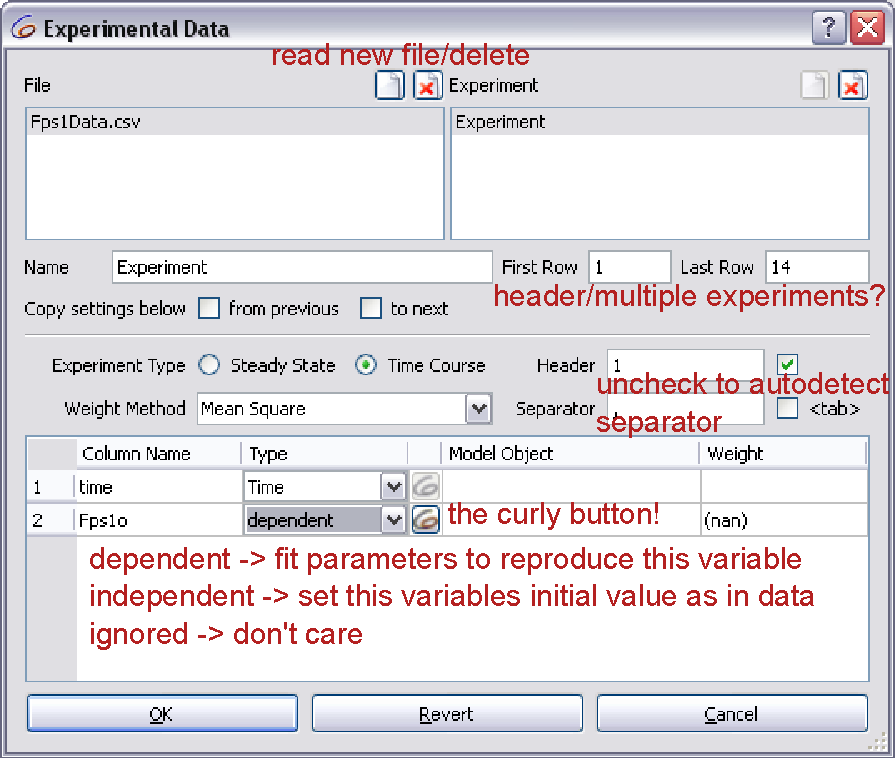
\includegraphics[width=09cm]{Pictures/ExperimentalData.pdf}
%  \caption{\footnotesize Settings for parameter estimation.}
%  \label{fig:PEdata}
% \end{figure}


\subsection{Stoichiometric Analysis}
\label{sub:sa}
The model structure of metabolic networks contains important information about the system.\\
\textbf{Elementary flux modes} show, which parts of the system can independently function in steady state. To use Elementary flux modes, the \textbf{stoichiometric coefficients of the reactions have to be integer numbers}.\\
\textbf{Mass Conservation} is used to check whether any the net output of the system equals the net influx. For glycolytic models, the standard analysis has to be used with care because not every molecule described  is  necessarily of  the  same  mass.  For  example, Fructose-1,6-diphosphate is cleaved into glyceraldehyde phosphate and dihydroxyacetone phosphate, producing 2 molecules from one without violating the factual mass balance.

\subsection{Metabolic Control Analysis}
\label{sub:mca}
Metabolic control analysis is a powerful theoretical framework to analyze the dependencies and regulation in biochemical models in steady state. Copasi can be used to compute three different measures of control:
\begin{itemize}
\item \textbf{$\varepsilon$-elasticities:} given all other parameters  remain constant, which effect will the change of a metabolite $S_i$ have  on the rate $v_k$ of a specific reaction?
\begin{equation*}
\epsilon_i^k = \frac{S_i}{v_k}\frac{\partial v_k}{\partial S_i}
\end{equation*}

\item \textbf{flux control coefficients:} given all other parameters  remain constant, how will a small change in reaction rate $v_k$ affect  the flux $J_j$ through reaction $j$?
 \begin{equation*}
 C_k^j = \frac{v_k}{J_j}\frac{\partial J_j}{\partial v_k}
 \end{equation*} 

\item \textbf{concentration control coefficients:} given that all  other parameters remain constant, how will a small change in reaction rate $v_k$ influence the steady state concentration $S_i$?
 \begin{equation*}
 C_k^i = \frac{v_k}{S_i}\frac{\partial S_i}{\partial v_k}
 \end{equation*} 
\end{itemize}
While elasticities are local properties, control coefficients are global quantities of the system: Even if a particular metabolite does not directly influence a certain reaction rate, its indirect effects are taken into account.


\newpage
\section{Exercises 1: A Simplistic Model for Cell Cycle Oscillations}
\subsection{Biology of the Cell Cycle}
A series of well timed events is needed to advance cells through their life cycle and allow them to grow and divide. In {\it Saccharomyces cerevisiae} (aka yeast), a model organism for the eukaryotes, the cell cycle can be divided into distinct phases (see Figure \ref{fig:CellCycleBio}, left) that are tightly controlled by the expression of specific cell cycle genes, the cyclins and cyclin-dependent kinases. Specific events take place in each phase and checkpoint mechanisms assure that everything is in best order before the cell commits irreversibly to the next cell cycle phase.\\
%
If the concentrations of the cyclins and kinases are plotted over time, an oscillatory behavior can be observed, which repeats the same pattern with a fixed frequency. We will see that even for the most simple system, dynamic dependencies are rather non-intuitive and, therefore, mathematical models are a powerful tool for dissecting the detailed functionality and timing of cell cycle regulation.\\
One of the most simple control systems for the cell cycle can be found in amphibian embryonic cells, where the accumulation of one cyclin compound is sufficient to trigger cell cycle progression. Goldbeter et al.\footnote{A. Goldbeter. A minimal cascade model for the mitotic oscillator involving cyclin and cdc2 kinase. Proceedings of the National Academy of Sciences of the United States of America, 88(20):9107–11, Oct. 1991} presented a first mathematical model with self-sustained periodic dynamics based on this system. It contains merely 3 agents: 
\begin{itemize}
 \item The cyclin {\bf C} itself, which accumulates steadily during the growth of the cell and at the same time triggers the activating dephosphorylation of
 \item the cdc2 kinase, also known as M-phase promoting factor {\bf M}. This protein triggers entry into cell division as well as the re-setting of the cell cycle by degradation of the cyclin. The degradation is facilitated by  
 \item the protease {\bf X} that needs the phosphorylation by cdc2 to become active.
\end{itemize}
\begin{figure}[h!]
 \centering
 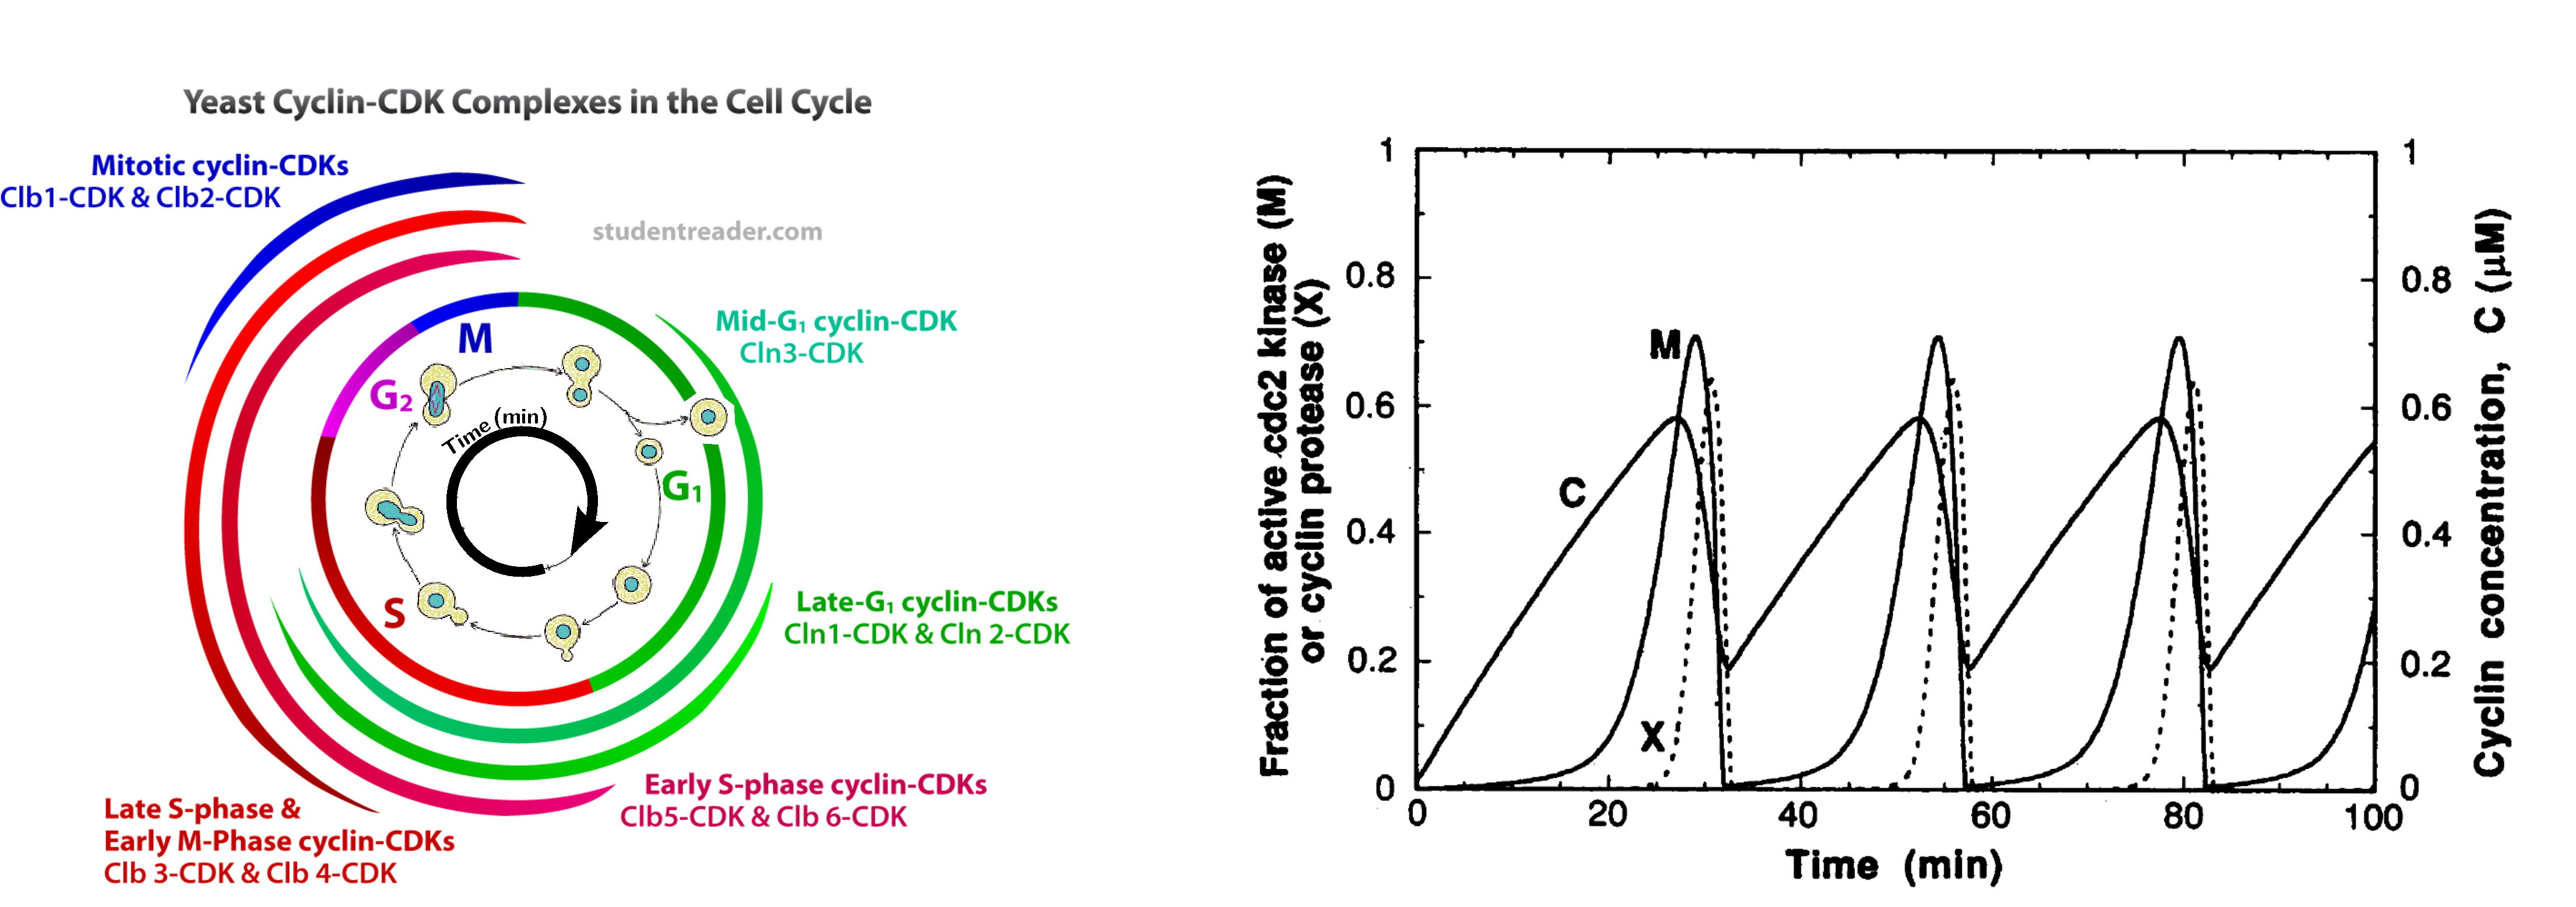
\includegraphics[width=\linewidth]{./Pictures/CellCycle.pdf}
 % CellCycle.pdf: 2122x683 pixel, 72dpi, 74.86x24.09 cm, bb=0 0 2122 683
 \caption{The cell cycle. \textit{left:} schematic representation of the cell cycle phases in yeast along with the expressed cyclins at each stage; \textit{right:} simulated cyclin dynamics of the Goldbeter model.}
 \label{fig:CellCycleBio}
\end{figure}

\newpage
The sustained oscillations in the model originate from the {\bf negative feedback loop} structure of the system along with activation thresholds for M and X. The thresholds are reached by a process called {\bf zero-order ultrasensitivity}, e.g. the level of activated M depends in an almost switch-like manner on the concentration of the cyclin. Hence, in the sensitive region of the cyclin concentration, small changes in C will result in large changes in M, whereas outside of this region changing C concentrations will have close to no effect.\\
These two conditions are sufficient to achieve cyclic behavior of the cell cycle components, as can be seen in Figure \ref{fig:CellCycleBio} on the right side.


 
\subsection{Goldbeter's cell cycle oscillator} 
Here, we want to apply our newly learned skills in Copasi to simulate a model of the cell cycle by Goldbeter \textit{et al.}. The model consists of a cyclin (C), a kinase (M) and a protease (X). The kinase and the protease have two states -- an active (M, X resp.) and an inactive one (M$^+$, X$^+$ resp.). The reaction scheme is given in \autoref{fig:goldbeter1}.
\begin{figure}[htb!]
\begin{minipage}{0.48\textwidth}
\centering
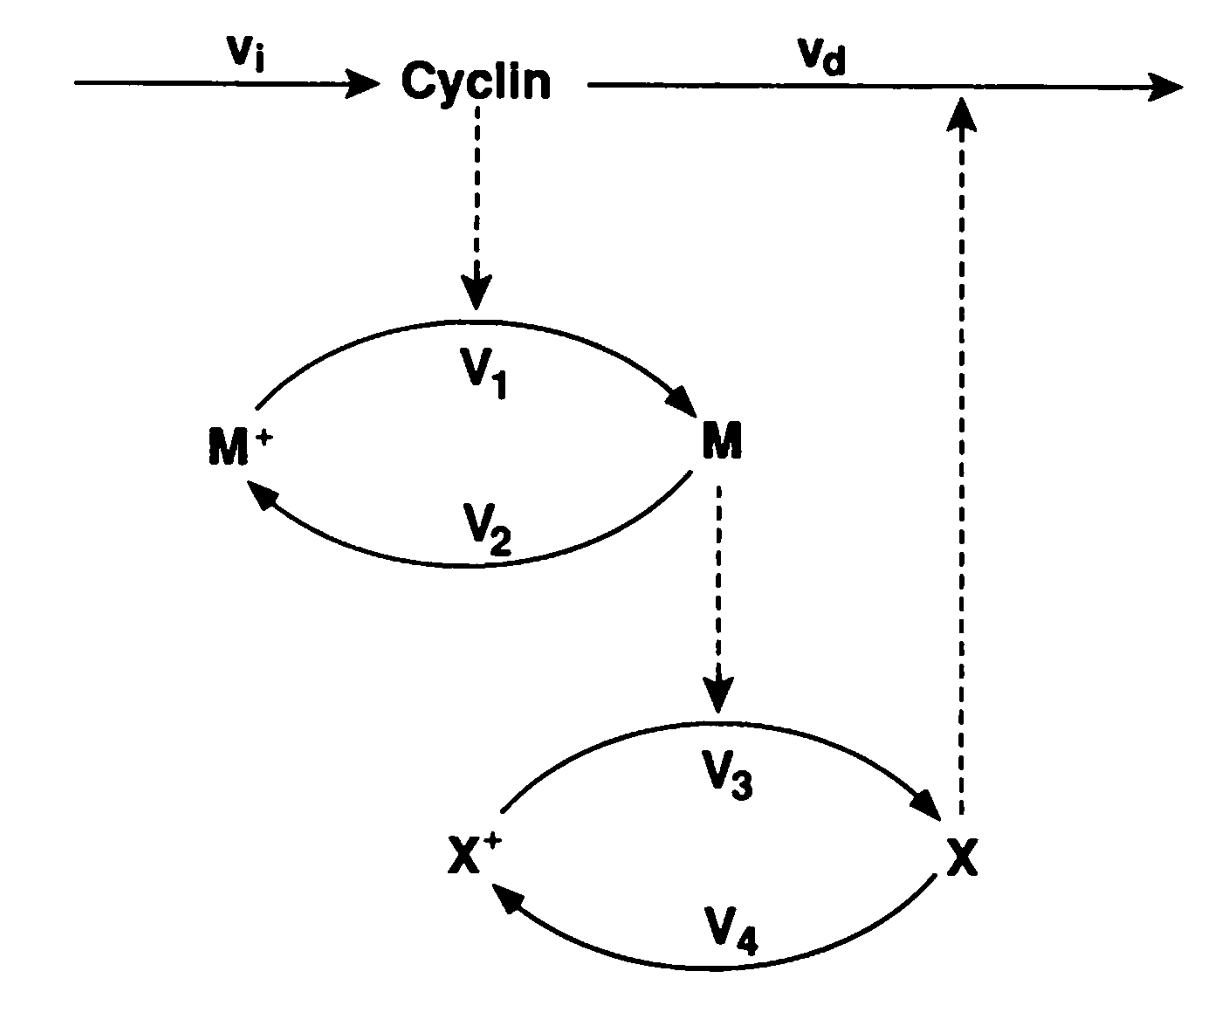
\includegraphics[width=\linewidth]{./Pictures/goldbeter1.pdf}
\end{minipage}
\vspace{1em}
\begin{minipage}{0.48\textwidth}
\centering
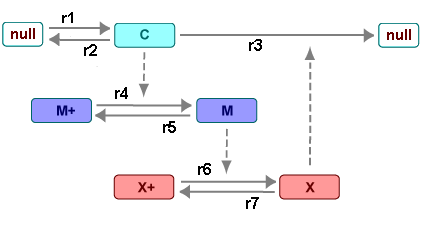
\includegraphics[width=\linewidth]{./Pictures/goldbeter_mitotic_oscillator2.png}
\end{minipage}
\caption{Reaction schemes of the Goldbeter model. \textit{left:} from the original publication \textit{right:} scheme for our implementation.}\label{fig:goldbeter1}
\end{figure}

\begin{enumerate}
\item \textbf{Model implementation}

\begin{itemize}
 \item Implement the reaction scheme according to Figure \ref{fig:goldbeter1} in Copasi. \\
Hint: Use mass action kinetics (Constant flux if not otherwise possible) to express the reactions \textit{r1} and \textit{r2}, and Michaelis-Menten type equations for the remaining reactions. You might have to define new functions.
 \item Parametrize the model arbitrarily and check if it can be simulated.	
 \item As in the original publication, we can assume that $M+M^*=1$ and $X+X^*=1$. Modify the reaction rates accordingly to obtain the following set of differential equations:
 \begin{enumerate}
 \item $\frac{\mathrm{d}C}{\mathrm{d}t}=v_i-v_dX\frac{C}{K_d+C}-k_dC$
 \item $\frac{\mathrm{d}M}{\mathrm{d}t}=V_1\frac{1-M}{K_1+(1-M)}-V_2\frac{M}{K_2+M}$
 \item $\frac{\mathrm{d}X}{\mathrm{d}t}=V_3\frac{1-X}{L_3+(1-X)}-V_4\frac{X}{K_4+X}$
 \end{enumerate}
 with $V_1=\frac{C}{K_c+C}V_{M1}$ and $V_3=MV_{M3}$.
 \item Extract the parameter values given in the publication to reproduce the original trajectories (Figure \ref{fig:CellCycleBio}, right side).
\end{itemize}

% \item \textbf{Model parameterization}
% We want to reproduce the model dynamics as given in the original publication, see Figure \ref{fig:goldbetersim}.
% \begin{itemize}
%  \item Use the data provided in GoldbeterSim.txt to fit the parameters.
%  \item Use 'Randomize Start Values' to test different start values.
%  \item Restrict parameter values to be larger than 0.001.
%  \item Restrict parameter values to be smaller than 5.
%  \item Use different algorithms.
%  \item Use the 'Parameter Scan' task to repeatedly test different random start values (don't forget to 'report' the results).
%  \item Could you use events to extract amplitude and frequency of each variable and fit those?
%  \item What else could you do to get working parameters?
% \end{itemize}

\item \textbf{Model visualization}
After you have obtained a sensible parameterization that leads to oscillations, visualize the oscillations:
\begin{itemize}
 \item Generate a phase plane plot of C vs M.
 \item Plot the phase plane for different initial conditions.
 \item Conduct a parameter scan (task: Time course) for one of the model parameters. Compare your results to the results of a sensitivity analysis for that parameter.
 \item Optional: Use events to extract amplitude and phase of the oscillation of each species.
\end{itemize}
\end{enumerate}


\newpage
\section{Exercises 2: Functional Analyses}

\subsection{Metabolic Control Analysis} 
 \begin{enumerate}
 \item Download the model BIOMD0000000253 from \url{www.biomodels.org} and open the associated article. Import the model into Copasi.
 \item Run the \textit{Metabolic Control Analysis} task and observe the matrix. What do positive and negative values mean in these three cases? Which flux and concentration control coefficients are strong? Can you relate this to the topographie of your model?
 \item Modify the model to describe unguarded glycolysis, rerun MCA and compare your results (you can also start a 2nd Copasi instance to better compare).
 \item Run the \textit{Sensitivities} task (time course subtask). To which parameters are the steady state concentrations (or a certain steady state concentration) in particular sensitive? Chose one of them and observe how the system reacts when changing this parameter (\textit{parameter scan}).
 \end{enumerate}
 

\subsection{Bistability:} Find and visualize bistability in a simple MAPK model.
 \begin{enumerate}
 \item Download and import BIOMD0000000027.xml from \url{www.biomodels.org} and read the model.
 \item Define an initial expression for the initial concentration for $Mpp$ of the form\\
 $Mpp(0) = 500-M(0)-Mp(0)$.
 \item Set up a plot with $MAPKK(t)$ on the x-axis and $Mpp(t)$ on the y-axis using symbols instead of lines for plotting.
 \item Run a \textit{Parameter Scan} over the initial concentration of $MAPKK$ using steady state as subtask and run 100 intervals from 0 to 100. Add another scan to the task, namely over the initial concentration of $M$, using 20 intervals from 100 to 450. What does the plot tell you?
 \item Add a third scan for the global quantity Km1, chose an interval from 50 to 500.
 \item The range of the bistable region in fact depends on the ratio between Km1 and Km2. Modify the model to enable a scan over this ratio. You can visualize the result in a contour plot with $MAPKK$ on the x-axis, Km2 (with fixed Km1) on the y-axis and $Mpp$ on the z-axis (color).
 
 \end{enumerate}
 

\subsection{Populations and evolution}
\begin{enumerate}
 \item Implement a model in Copasi  that considers the reproduction and degradation of some population $pop$. Reproduction requires consumption of $food$, which is able to reproduce itself.
 \item Find a parameterization that gives classic predator-prey dynamics over a given time.
 \item Introduce a second population $pop_2$ that either growths faster or dies slower. Find the parameter values for which $pop_2$ out-competes $pop$ within a certain time range:
  \begin{itemize}
    \item Create a global variable that is the difference between $pop$ and $pop_2$
    \item Use the \textit{Parameter Scan} and an appropriate plot output to define the critical value where the behavior switches for each parameter.
 \end{itemize}
\end{enumerate}

% \begin{enumerate}
% \item \textbf{Parameter Estimation:} A lab sends you absorption data  for the characterization of an enzymatic reaction (mmspect.txt). The  reaction follows Michaelis-Menten kinetics  (E + S = ES, ES  $\rightarrow$ E + P). Enzyme concentration used is $0.01$ in all
%  experiments.
%  \begin{enumerate}
%  \item Implement the according mass action reactions.
%  \item Should the enzyme concentration by fixed or does your model
% ensure that the total enzyme concentration remains constant?
%  \item Fit the parameters to all experiments. Before you start
% fitting, you should consider the following:\\
% \begin{itemize}
% \item The absorption values measure the amount of P produced
%  according to the formula $\textrm{Abs}=P\cdot \textrm{coeff} +
%  \textrm{offset}$, where $\textrm{coeff}=0.78$ and
%  $\textrm{offset}=0.027546$.  You can use the data directly,
%  without having to change the data table. How?
% \item In the parameter estimation dialog in Copasi, you can set
%  'independent' variables. These are the not used for fitting but
%  set to the value specified in experimental data. Can you use
%  this to automate/ease fitting?
% \item Importing experimental data for
%  different experiments is facilitated using the 'copy settings
%  below from previous/to next'.
% \end{itemize}
%  \end{enumerate}


% \subsection{Protein multimers and parameter estimation}
% \begin{enumerate}
%  \item Consider a protein that can reversibly form dimers and trimers (from a dimer and a monomer), and implement this in Copasi.
%  \item Estimate the parameter values and initial values that reproduce the data given in Table \ref{tab:protdata}.
% \end{enumerate}
% 
% \begin{table}[htb]
% \begin{center}
% \begin{footnotesize}
% \begin{tabular}{l|rrr}
%  Time (s)&monomer &dimer &trimer \\
%  \hline
%  0.1& 38 &20 &30 \\
%  0.5& 30 &18 &33 \\
%  1& 25& 21 & 35\\
%  1.5& 21 & 19 & 36\\
%  2& 18& 19& 37\\
%  3& 14& 19& 40\\
%  5& 8& 17& 42\\
%  7& 6& 15& 44\\
%  10& 4& 14& 46
% \end{tabular}
% \end{footnotesize}
% \end{center}
%  
% \caption{Experimental data for the protein multimer exercise.}
% \label{tab:protdata}
% \end{table} 

% \subsection{Model creation:} Consider the system\footnote{extracted from Mirams  G, Byrne  H, King
% J. \textit{A multiple timescale analysis of a mathematical model
%  of the Wnt\/$\beta$-catenin signalling pathway.} \textbf{J Math
%  Biol} 2010; 60(1):131--160} composed of a species $X$ that
%  changes over time due to the signal $W$, and that is represented with
%  the following ODE:
%  $$\frac{dX}{dt}=v_{12} -(a(W(t))\cdot\frac{K_{17}}{K_{17} + X(t)}+
%  k_{13})\cdot X(t)$$
%  The variable $W$ is time-dependend. The function $a(W(t))$ defines
%  the role of $W$ in the rate of the reaction to $X$. It has a
%  Michaelis-Menten dependence on $W(t)$:
% $$a(W(t))=2.806 \cdot 10^{-3}\cdot(\frac{W(t) + 0.1}{1.075 \cdot W(t) +
%  0.0165})$$
%  \begin{enumerate}
%  \item Implement this system in Copasi (implement X and W as species, and
% a(W(t)) as global quantity). The values of the parameters are
% given below. Pay attention to the units.\\ ~\\
% \underline{Model parameters:}\\
% $v_{12}= 0.423 nM \cdot min^{-1}, k_{13}= 2.57 \cdot 10^{-4},K_{17}=
% 1700$,\\
% $X=25 nM, W(t)= e^{(-t/20)}$.\\
% ~\\
% Verify that your reactions give the same ODE as above
% (``Mathematical - Differential Equations''). Then, run a ``Time
% course'' with deterministic simulation, for 1000 minutes, and
% observe the dynamics of X.\\
%  
%  \item Indeed, the initial concentration of X is 35 nM, 25 nM is the
% concentration at the steady state. In order to observe the dynamics, you will change the model as follows:
% \begin{enumerate}
% \item add a condition for W: if $t<0, W(t)=0$, else it remains as
%  before.
% \item set the initial concentration of X to 35 nM.
% \item set the initial time of the model to -300 minutes.
% \end{enumerate}
%  \item Run a time course of 1000 minutes and observe the curves for X
% and W.
%  \item Put back the initial time to 0. A lab send you the
% kinetic results of X over time (kinetics.txt). Fit your
% model to the experimental data.\\ ~\\
% \underline{Tips:} add lower and upper bounds (e.g. $0 \le k \le 1$,
% or $0 \le k \le 10000$)\\ ~\\
% Update the model with the parameter values extimated: are the
% simulation results close to the experimental ones?\\
%  \end{enumerate}
% 


% \end{enumerate}





\end{document}

